\documentclass[a4paper,12pt]{extarticle}
\usepackage{graphicx}
\usepackage{amsmath}
\usepackage{a4}
\usepackage{algorithm}
\begin{document}
\title{THE ENGINE BEHIND MODEL CHECKING}
\maketitle
\begin{center}
\textsf{
PROJECT DISSERTATION SUBMITTED FOR PARTIAL FULFILMENT FOR THE DEGREE OF MASTER OF SCIENCE \\ by \\ 
}
\textbf{Reema S Patne \\ MSc. In Computing and Software Technology \\ Swansea University}
\end{center}
\newpage  
\begin{abstract}
\textsf{In order to ensure the safety and quality of a system, it is necessary to undergo a process of system validation which checks the correctness of specifications, designs and products.\cite{Berardetall2001} We find post-completion errors which are a particular kind of error in interactive systems. When there is an incorrect sequencing of goals and sub-goals, this type of error occurs. Mainly because, the primary goal is achieved before all of the prerequisite sub-goals have been satisfied. This project shows how we can check for this property in a formal model of an interactive system. Of all the validation techniques, model checking has become the most popular approach in the both hardware and software areas due to the availability of various support tools and its success in the project. This project is to get a working understanding of a model checking tool that uses SAT solvers. Specifically, suggesting the lightweight formal methods, such as the Alloy structural modelling language, is particularly well suited for this task. As a case study we develop an example interactive system using ubiquitous coffee machine where both coffee and change must be delivered.}
\end{abstract}
\newpage
\begin{center}
\textbf{Acknowledgement\\}
\end{center}
\textsf{ \\ My foremost thank goes to my thesis supervisor Dr. Oliver Kullmann. Without him, this dissertation would not have been possible. I thank him for his patience and encouragement that carried me on through difficult times, and for his insights and suggestions that helped to shape my research skills. His valuable feedback contributed greatly to this dissertation.\\ I thank all the students and staffs in the Computer Science department, who taught me knowledge and helped me with my study and life in Swansea University. Especially I thank several good friends of mine, who always encouraged and supported me.\\ Last but not least, I thank the Almighty, my parents and all other family members for always being there when I needed them most, and for supporting me throughout the years.}
\begin{flushright}
Reema S Patne\\
MSc in Computing And Software Technology\\
Swansea University\\
September 2012.
\end{flushright}

\newpage 
\tableofcontents
\maketitle
\newpage
\section{Introduction}
\label{Intro}
\subsection{Problem Statement}
\label{prob stat}
Interactive systems are prone to the common types of errors like the one similar to the specific behaviour of cash machine who leaves back their cash card in the ATM machine after the cash is withdrawn. Also, like the ones retrieving the photocopies from the Xerox but forgetting to collect the original document is another common error with the interactive systems. This type of error is referred to as a``Post Completion" error.[finally] Achieving the primary goal even before all the sub-goals are satisfied is the key characteristics of these errors. In other words, the main objective is achieved but, due to the wrong sequencing of events we forget to do the items that were before it on the list. These kinds of errors usually don't occur, but however we should try the every possible way of preventing these kinds of errors from occurring. This kind of errors can be handled by ensuring that sequences of sub-tasks are completed before the main goal is achieved at the end of the sequence. The various interactive errors can be checked by correctly formulating the problem and using the existing formal method tools. This error can be approached by using the lightweight formal method, namely Alloy which uses the SAT solvers, where the constraints in the Alloy -a declarative modelling language, can be translated into Boolean logic and solved with the SAT solver.But the project focuses on the SAT translation and not on the  SAT solver which is a black box for the project. The presented approach is explained with help of an example coffee machine. This project demonstrates how the Alloy Analyser which is used as a SAT translation to conduct fully automated analysis of a coffee machine specification represented in Alloy. \\
The Alloy Analyzer is a compiler which translates the problem to be analyzed into a (usually huge) Boolean formula. This formula is then handed to a SAT solver, and the solution is translated back by the Alloy Analyzer into the language of the model. The Alloy Analyser thus makes the problem finite (and reducible to a Boolean formula) by solving the problems within a user-specified scope that bounds the size of the domains. In otherwords, model-finder essentially translates a model expressed in relational logic into a corresponding Boolean logic formula, and then invoke an off-the-shelf SAT-solver on the Boolean formula. In the event that the solver finds a solution, the result is translated back into a corresponding binding of constants to variables in the relational logic model
Although the analysis can be performed by a traditional formal method, there is a lower barrier to entry afforded by lightweight formal methods.\\
The lightweight formal methods such as Alloy provide the user with many benefits:
\begin{itemize}
\item   In order to develop an ongoing development, the formal basis provides an automatic feedback in a more focused way.
\item   Tools provide a more ``programmer-friendly" interface and can be used by any developers who are not formal methods experts. [finally]
\item • In software engineering, one of the great benefits of Alloy is that you can analyze a tiny model, write three lines, and analyze it, add few more lines and analyze again. This increment makes Alloy especially good for exploring design ideas. 
\end{itemize}
These approaches are used much earlier in the development process to validate aspects of an evolving specification and to explore requirements. Here the focus is on post-completion errors as an example property but is chosen only to serve as an example and our models are not designed solely for any particular property. The models are general and able to be used to investigate many other properties.\\
In this dissertation, the literature survey, specification, implementation of alloy Analyser, example using Alloy, conclusion of the model checking tool will be presented.
\subsection{Outline Of This Dissertation}
\label{Outline dissert}
This report mainly consists of three parts. Part I is the literature survey, Part II is the Specification and part III is the Final thesis.\\
In Part I the concept of systems and their specifications and the basic theory of model checking technique will be presented. A simple example to illustrate the technique is mentioned. The various model checkers along with their uses are listed. The new challenges faced throughout the project are also mentioned along with the conclusion of the literature survey.\\
In Part II the discussion of making the specifications executable will be found. The approach which is used to make the specification executable will be discussed. It introduces the declarative modelling language namely Alloy followed by development and analysis of a Alloy model which includes alloy interface walkthrough also introducing the Alloy's improved solution visualizer. It also includes the schedule of the project planned throughout the course.\\
Finally the Part III examines an Alloy model which solves the coffee machine problem, using the module for modelling the ordered state. It will conclude with the method, result and refinement along with the references. 
\pagebreak 
\part{LITERATURE SURVEY}
\pagebreak 
\section{Model Checking}
\label{Model check}
The technique used for validating a system is Model checking. The design process and the validation process are the must to ensure the correctness of specifications, designs and products of the system. Validation is done to see that whether the system meets all its requirements. \\
The two types of validation techniques are: 
\begin{itemize}
\item   Informal ones which include peer testing and testing.
\item   Formal ones which include formal verification, simulation and model checking. 
\end{itemize}
This report focuses on the Formal validation technique – Model Checking. \\
Model checking systematically checks the validity of a given finite-state model of a system and properties stated in the form of logical formalism such as temporal logic. It uses algorithms which are executed by the computer tools. The inputs to such model checkers are the description of the model and the description of the properties. Once these files are fed as an input, the model checker performs the verification. If error occurs, then the model checker provides the counter-example to explain under which circumstances the error can be generated. This counter-example helps in finding the error and repairing the specifications of the model. This can be shown with help of the following diagram. It shows us how the verification process takes place in the model checking.  \\ 
Describing what a system is required to do is known as system specification. By doing so, we will be able to understand the system. Various validation techniques are used to check the correctness of specification. It guarantees the quality of the system and also its safety [8]. Model checking is one of the most popular validation techniques. For a system defined in finite state model and a property defined in terms of logical formalism, model checking techniques could systematically check the validity of this property [15]. A finite-state model is used to design computer programs and digital logic circuits. It is as an abstract machine that can be in one of a finite number of states. It will be only in one state at a time; the state it is in at any given time is called the current state. When initiated by a triggering event or condition, the state changes, this is called a transition. \\
Roughly, M is an abstract model of a system whose structure is defined as finite-automata and $\phi$  is a logical formula specifying a desirable property such that M satisfies $\phi$  abbreviated as $M \models \phi$. \\
Model checking helps from preventing the bugs even before penning down the code of the project i.e., during the requirement and the design phase itself. It prevents the further breed of the bugs and hence it makes sense by being cost effective [7]. The errors which are not been able to find by simulation is done by model checking by considering all possible behaviours of the system[3]. \\
Model checking is the one of the foremost applications of logics which ranges from computer science to computer engineering. Since then, there has been a multiple breakthrough. The gap which was built between the theoretical computer science, hardware and software engineering was bridged by Model Checking. Now, model checking has been extensively used for verifying many Software and also used in hardware industry. It has virtually became a universal tool for the analysis of the systems. Henceforth, this project will focus on the state of the art of model of model checking.
\subsection{Systems and their Specifications}
\label{Sys and Spec}
Describing a system is called specification. Specification helps in finding errors and    understanding a system. So, it is a good practise to have a clear idea about the design and improve it before the implementation. The specification of the system can be functional or non-functional i.e. what a system is supposed to do or performance properties. These specifications are written in formal language with proper syntax and semantics which can be verified and validated with respect to requirements.\\ 
It helps in developing the explicit model of a system which is clear, precise and unambiguous. Mathematics is used as a basic tool to achieve this. Here, reading the accompanying words in order to understand the relation between the equations is a bit tedious. In order to overcome this shortcoming using mathematics as a basic tool, logicians have temporal logic which is precise and completely formal mathematics. This temporal logic is used in such a way so as to describe the system behaviour. 
\subsection{Temporal Logic} 
\label{Temp Logic}
There are various interpretations of temporal logic depends on the individual as how to consider the system with time. It is the logic for expressing mathematics. It supports formulating the properties of the system behaviour with respect to time. There are various types of temporal logics:
\begin{itemize}
\item • Temporal Logics used to specify the reactive systems are: \\
\textbf{Linear temporal logic:}It allows the statement of properties of execution sequences of a system. \\
 \textbf{Branching temporal logic:}It allows the user to write formulas which include some sensitivity to the choices available to a system during its execution.
\end{itemize}
These two kinds of temporal logic are characterized by a continuous interaction with the environment [15].
\begin{itemize}
\item • Temporal Logics used to specify the time-critical systems:\\
 \textbf{Real-Time temporal logic:}  It allows statement of properties of multiple concurrent processes and supports relative time references.
\end{itemize}
It is characterized by quantitative timing properties relating occurrences of events [15].
In order to avoid the errors we write specifications. Validation techniques are used to checking the correctness of the system.  \\
\subsection{Model-Checking Algorithm}
\label{Model chec Algo}
Model checking uses exhaustive state space search of the system model as        algorithm: The desired properties satisfied for each state of the model.        Reachability property is used to check whether the system can reach a state without any deadlocks. Reachability is considered as one of the important property which uses Reachability analysis technique. It starts from initial system state and see to it that it reaches all the possible system states which can be reached. For instance, in a traffic signal model, yellow, red and green are the three states. Model checking proves if it can reach some state, all the states are eventually got by the model, or if the model could never get some state.
\subsection{Approaches Of Model Checking}
\label{Appr to model check}
\begin{itemize}
\item Logic based approach: Here the system is modelled as finite-state automaton representing the states as values of variables and control location, and changes of a system from one state to other state is represented by transition. If a system satisfying the desired behaviour given in some logic with the initial set of states, then the system is said to be correct.
\item Behaviour based approach: Given the desired and the possible behaviour with the same notation, the equivalence relations are used as criteria for the correctness. Hence, if the desired and the possible state behaviour are equivalent then the system is said to be correct.  
\end{itemize}
\subsection{Model Checkers}
In verifying a system, model checking techniques uses tools known as model checkers. Due to the progress of model checking, industries are developing their own model checkers. 
Exhaustible list of  Model Checkers are given below:
\begin{description}
\item[Blast model checker:]Berkeley Lazy Abstraction Software Verification Tool abbreviated as BLAST .It is a model checking tool used for C programs.
\item[CADP:]Commonly known as  Construction and Analysis of Distributed Processes.It uses the formal description technique and software tools for simulation to facilitate the design of reliable systems.
\item[Chess model Checker:]It is a software which uses thread schedules to find bugs or errors in multi-threaded software such as deadlocks,data-corruption which are hard to find using testing tools.It helps in debugging the process by providing the full repeatable execution of the program which is causing an error.
\item[CHIC:] Commonly known as Checker for Interface Compatibility. It is used in hardware and software systems to verify the behavioural compatibility.
\item[FDR:] Commonly called as Failures-Divergences Refinement is the software tool used to check  the refinement.
\item[ISP:] Commonly known as In-situ Partial Order .It is a formal verification tool.They perform the verification at the level of code.It has successfully verified the codes for deadlocks and assertion violations.
\item[Java pathfinder:]The executable Java byte-code programs are verified by this Java pathfinder system.It does the model checking for the concurrent programs.As using this it helps in detecting the deadlocks and data races.It can also be used to model check the distributed applications and user interfaces.
\item[LTSA:] It is commonly known as Labelled Transition System Analyser. It is used to verify the concurrent systems. FPS process algebra is used to describe LTSA. The systems are finite state machines.
\item[MRMC:] Commonly known as Markov Reward Model Checker is tool written in C programming language.It model checks for discrete-time models and continuous –time model.Within a given time and within the constraint it checks the reachability of the set of goal states.
\item[mCRL2 Toolset:]It is used to describe the concurrent systems since it uses the specification language.
\item[MoonWalker:]It model checks for .Net applications by detecting the errors.Also it is able to find the deadlocks and assertion violations as well.
\item[NuSMV:] It is the expansion of  symbolic model checker.It provides verification for industrial designs.Also it provides analysis of specifications.
\item[Ompca:]It is commonly known as Open MP C Analyser .It helps in model checking  real-time systems with dense-time models.It is an application for timed automata’s.
\item[PAT:]It is commonly known as process analysis tool kit.It helps concurrent and real-time systems in reasoning and simulating.It helps in solving deadlocks and reachability.
\item[PRISM:]It is commonly called as probabilistic model checker.It is used in model checking for the system that exhibits probabilistic behaviour.This software tool is used in modelling and analysis of the system.
\item[Rabbit:]It does model checking by providing the reachability analysis and refinement.It is used for real-time systems.
\item[REDLIB:] It is a model checker for timed automata’s.It helps in verification tasks.
\item[SMART:] It is a model checker used to check the reliability and timing.
\item[Spin Model Checker:]It verifies the correctness of the models in automated fashion. This is one of the biggest achievements. It avoids pre-construction of the states.
\item[TAPA’s:]It is a tool used in concurrent systems for specifying and analysing.It also helps in model checking temporal formulas.
\item[Vereofy:]This model checker checks for operational correctness .It model checks for component-based systems.
\item[mCRL:] It studies description and analysis of distributed systems.It solves the problem in a very simple manner using the algebras CCS,CSP and ACP.
\item[UPPAAL:]It is used for real-time systems for modelling,validation and verification.
\item[Romeo:]This is same as UPPAAL which is used for modelling,validation and verification of the real-time systems.
\item[TLA+:]It is commonly called as Temporal Logic Of Actions.It combines logic of actions with temporal logic.In concurrent systems TLA+ is used in describing its behaviour.
\item[AlPina:]It is commonly called as Algebraic Petri Nets Analyser.It provides model checking for algebraic petri nets.
\item[McErlang:]It is a model checker used in checking the programs written in erlang language.
\end{description}
\subsection{Technology}
\label{tech}
Model checking then, used explicit state traversal where the reachable state space was traversed to find the errors violating the safety properties. It consumed lot of space in the computer memory because each state of the system was stored in large hash table. In order to improve this space consumption in explicit state model checker various techniques came into existence. SPIN model checker was the most successful explicit model checker. The goal of this was to overcome the state explosion problem where the states of the model were represented symbolically. 
Later in mid-80's Binary Decision Diagrams as a new data structure came into existence for symbolical representation and manipulating Boolean functions efficiently [4] known as Symbolic model checking with BDDs. BDDs could handle much larger designs with hundreds of state variables representing Boolean functions. There existed some shortcoming in BDDs as well. They became too large to handle as they used canonical representation. BDDs required uniform variable ordering along the paths and it sometimes happened that no space efficient variable ordering existed. This was time consuming and needed manual intervention. 
There came into existence the SAT procedures as an alternative approach to model checking. Unlike BDDs, it didn’t use the canonical representation. It became one of the most efficient implementation. It overcame the state explosion problem faced by BDDs. 
In late 90s, researchers came up with the idea of Bounded model checking which uses SAT solvers to the model checking problem. Bounded model checking technique do a fast exploration of state space overcoming the shortcomings of the previous approaches using the SAT procedures instead of BDDs where the SAT has a depth first search nature. This method is applicable for properties which include safety and liveness where it checks whether a given set of states is reachable, and detects loops in a system’s state transition graph.
\subsection{Example to illustrate the new technique}
\label{Example}
Application of Model Checking ranges from simple coffee machines to nuclear plants which are undoubtedly critical and the failure of which may cause economical and physical damages. Considering an example of a coffee machine, where the system is fed with a sensitive data to check the behaviour of the system as it is supposed to behave. This is known as testing. 
 \begin{figure}[h!]
 \centering
 % 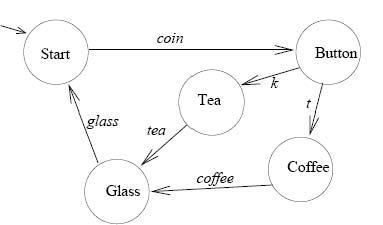
\includegraphics[width= 0.5\textwidth]{flower.png}
\caption{Finite states of a coffee machine.}
 \end{figure}
 A coffee machine consists of a set the following above states which are depicted in circles and relations as arrows between the states. Arrows are given with labels representing actions. The combination of this set of states and relations is known as ``automaton".  If the given action on an arrow connecting both the states is satisfied, then automaton in a given state changes to another state. 
Initially the machine is at state ``Start" and it ``waits" for a coin. If a coin is provided then the machine change state to the ``Button" state where two options are possible: to press the ``k" button and then go to the ``Coffee" state, or to press ``t" and go to the ``Tea" state. After serving the corresponding drink, the machine goes to the "Glass" state and it gives a glass with the chosen drink to then go back to the ``Start" state.
\paragraph{Example 1}
The property ``Always, after the machine gets a coin and the user press a button, it gives coffee or tea", can be written in temporal logic as:
ALWAYS (IF Button THEN (SOMETIME-IN-THE-FUTURE (Coffee OR Tea)))
Words in upper-case are temporal logic ``connectives" or ``operators", and the other words represent the interaction between the machine and the user. The above expression is a ``formula" of temporal logic.
How can one see that the given automaton satisfies a formula? We can explain it by using the above formula and the automaton modelling the coffee machine.
Let us assume the current state of the automaton is the initial ``Start" state. Let A and B be statements, then ``ALWAYS A" means that A must be true in all the states of the automaton. ``IF A THEN B" means that whenever A is true in a given state, so is B. ``A OR B" means that at least one of A and B must be true in the state. Finally ``SOMETIME-IN-THE-FUTURE A" means that it must exist a state in the future of the current state where A is true.
It is then possible to check that the above formula is satisfied by the automaton, since from the state ``Button" (after a coin is inserted) it is possible to find a state in the future such that the actions ``coffee" or ``tea" are possible.
\paragraph{Example 2}
Let us consider now the following property: ``Always, after pressing a button the machine will serve coffee and then tea immediately afterwards". We can write this sentence as follows:
ALWAYS (IF Button THEN (Coffee AND NEXT Tea))
Here NEXT is a connective formalising the ``immediately after" English expression. As for the previous example it is possible to check whether the automaton satisfies the property. In this case we can see that it is not the case, since from the state ``Button" one can reach the state ``Coffee" and ``Tea", but from the ``Coffee" state it is not possible to go immediately after to the ``Tea" state. This property guarantees that the machine will never allow to get coffee and then tea by paying only once.
\section{Challenges Faced}
\label{challenge face}
\begin{itemize}
\item Learnt the usage of Github: It is a website used for storing and presenting our files. Git is a decentralized version control system that is used by a number of open source projects, most notably perhaps the Linux kernel. GitHub is a new hosted Git repository service that's being called a "social network" for programmers and with good reason. In my project it helps in communication between me and my supervisor by providing information to assist in evaluating the tools and making an informed decision.
\item Learnt the usage of LATEX: It is a document preparation system similar to that of a Microsoft word where the similarities end here. Preparing a document with LATEX consists of using a text editor to edit a Latex source file with the .tex extension. And then running a latex program to convert the source file to a document interchange format like PDF etc. Doing in LATEX provides a good typography which provides a good impression on the content of the document and is platform independent unlike MS word which runs only on windows. It's much better than copy+paste since it can be changed by changing just the definition. Even more, Latex allows people to write programs in their documents. 
\end{itemize}
\section{Conclusion of literature survey}
Model checking is used in many areas including both the hardware the software fields. It helps in considering only subset of the system requirements leading to the improved efficiency by supporting partial verifications. Compared to simulation and testing, model checking uses shorter time for verification as shown by many case studies. It can also deal with the states which are larger. \\
There are shortcomings that still need to be answered:
\begin{itemize}
\item   There is no way to translate automatically the requirements into its own modelling language defined by its model checking tool. This has to be done manually.
\item   Some of the properties which are to be verified are difficult to express in the notation.
\item Model checking involves much number of states consuming extra efforts in checking parts of the model separately. 
\end{itemize}
Despites these shortcomings the model checking is an important and successful area in verifying the models by early detection of the errors [3].
\newpage 
\part{SPECIFICATIONS}
\newpage 
\section{Making the Specifications Executable}
\label{Spec exec}
It is difficult to validate the system with the specifications and requirements. The     validation task would be easier if we make the specifications executable, giving the immediate feedback of the behaviour of the future software to the user.\\
The Boolean level of representation of the model-checking task with the   computation engine that supported the required set of operations gave rise to Symbolic model checking. Ordered Binary Decision Diagram (OBDD) was the first approach combining the efficiency and expressive power. Recently, based on Davis-Putnam-Logemann-Loveland (DPLL) algorithm, Boolean satisfiability (SAT) checkers have greatly extended the reach of bounded model checkers.\\
OBDDs and DPLL –based checkers compliments each other. OBBDs readily deal with quantified Boolean formulas (QBF) where as DPLL cannot. SAT problem which are completely intractable for DPLL are trivial with OBDDs. SAT checkers are insensitive to the number of variables. 
\subsection{A view from the Engine Room}
\label{View from engine}
The first symbolic model checkers used Ordered Binary Decision Diagrams (OBDDs) [5] to represent system transition relations and sets of system states [2]. All the steps required for a model checking is expressed as a series of operations on these representations, without enumerating individual states or transitions. Recently, Bounded and Inbounded model checking has been devised which use Boolean satisfiability (SAT) solvers as a computational engines. Combining the methods which have a SAT solver work on a detailed system model and OBDDs operate on a abstracted model, is more powerfull than operating on its own[8].\\
Model checkers are now able to handle the complex verification problems coming from real world hardware and software designs with the help of Boolean methods. By giving the importance of Symbolic model checking, I take this opportunity to examine the capabilities of SAT solver.
\subsection{Experiments in (Un)SAT}
\label{Expt in UnSAT}
When the given task is to prove that the given formula is unsatisfiable, we find an error in the design by using the SAT solver which is typically used by verification problem. To prove that the formula is unsatisfiable, it is currently highly favourable to use DPPL method [13].for solving SAT problems by backtracking search among complete SAT algorithms. By doing so, it has gained a remarkable progress in speed and capacity[14].\\
I would like to be working on the use of Alloy as the formalism used for the formal analysis of models.. Alloy is a lightweight modelling language for software design. By using the Alloy Analyzer, it is amenable to a fully automatic analysis. It also provides a visualizer for making sense of solutions and counterexamples it finds.\\
Alloy can be considered as a natural choice for representation of interactive systems.  The remainder of the project will be structured as follows: Firstly, introducing the key concepts of Alloy. Then, describe the approach of analysing the model with the Alloy Analyser and applying it to an example. 
\section{Alloy Language and the Alloy Analyzer}
\label{Alloy and its Analyzer}
To facilitate the lightweight modelling object, Daniel Jackson, with the    assistance of others at the Software Design Group, a declarative modelling language was designed. It allows for writing Z-style specifications in ASCII, and, being close to first-order, is analyzable via translation into SAT . A platform is developed to perform this analysis which is known as Alloy Analyser.
Specification of Alloy consists of signatures, facts, functions, predicates and assertions. 
Signatures declare the types used in the specification, and the definitions of the types fields. Types in Alloy are hierarchical in the form of a tree; a type may have multiple subtypes but at most one supertype. In addition, all types descend from a common ancestor, which is called univ. The types and fields defined in signatures form the set of relations that are used in the specification. \\
Facts are logical formulae or constraints over relations. They may be nested via standard logical operators, such as disjunction , conjunction , and negation . The value of a formula is thus always Boolean. \\
Predicates are logical formulae that are evaluated on zero or more arguments. They can be called within the model or used to run an analysis of the model. Given a predicate to analyze, the Analyzer finds a solution that satisfies both the facts and the predicate, or returns that no such solution exists (within the given scope bounds, which are discussed in the next section). \\
Assertions are logical formulae whose validity we want to check. That is, given the signatures and facts, we want the Analyzer to help us determine whether an assertion always evaluates to true, and if not, provide a counterexample that demonstrates otherwise. The natural way to do this is to conjoin the facts of a specification with the negation of the assertion, and translate this compounded formula into SAT. If no solution can be found, then this means that the assertion is always true when the constraints are true (within the given scopes), or that the constraints are inconsistent and always false. The latter case implies a faulty specification. On the other hand, if a solution is found, then it illustrates a counterexample case in which the constraints are true, but the assertion is false. 
Describing some aspects of a system (but not the entire system), constraint it to exclude ill-formed examples and checking the properties about it is the main goal of writing a model. The property of allow always holds for problems up to size X or if the property does not hold good, it provides a counterexample. \\
The two kinds of problems that may occur are:
\begin{itemize}
\item   Bugs: It occurs in the model itself. The problem of overconstraining and underconstraining our model will be discussed and how to eliminate those bugs.
\item It occurs in the subject we are modelling. These are what we are after, and what the modelling is all about. The example will also show how to make and check assertions about our systems, and how to track down why a given assertion failed to hold. 
\end{itemize}
Apart from the similarities of Alloy with other existing languages and modelling techniques, there are several other differences as well:
\begin{itemize}
\item   Finite scope check: After analysing the model, the scope (size) must be specified to the model. The analysis is sound and it never returns false positives, but incomplete because it checks the things only upto a certain limit. However it is complete upto the scope. Counterexample being smaller than the specified scope is never missed. Smaller scope checks are extremely valuable for finding errors. 
\item Infinite model: Unlike traditional model checking models written in alloy do not reflect that analysis is finite. That is, components of the system and how they interact will be described, but do not specify as to how many components there can be. 
\item Declarative: As opposed to ``operational" or ``imperative" modeller which asks ``How can I accomplish X" , a declarative modeller answers the question ``How would I recognise that X has happened".
\item   Automatic analysis: Alloy can be automatically analyzed unlike some other declarative modelling languages like Z and OCL, the object language of UML. Examples of the system and the counterexamples to claims made about the system can be generated automatically.
\item Structured data: Alloy is a rich way to describe states by supporting the complex data structures, such as trees.
\end{itemize}
\section{Boolean translation of the Alloy constraint}
\label{Bool Transl}
By placing a bound on the universe of atoms, we will be able to solve the constraints in first-order logic. By doing so, the search space becomes finite and then translating the constraints into the Boolean form finally finding the solution with a SAT solver. The SAT solver finds a solution to the satisfiability (SAT) problem: \\
Given a Boolean function f(x1,..,xn), return an assignment of Boolean values to xi such that f evaluates to true, or prove that no such assignment exists. The solution is mapped back to the original constraint problem in a manner comprehensible to the author of the constraints. \\
 For our project, it is only necessary to have a basic understanding of how the translation into Boolean logic works in Alloy. \\
``The universe of atoms is bounded by a user-defined or inferred scope for each type used in the object model. Consider a binary relation 
\begin{equation}
r : X->Y
\end{equation} with the scopes of X and Y set to m and n, respectively. Then, r can be represented as an m-by-n Boolean matrix where a value of true in the i-th row and j-th column means that the i-th element of X is related to the j-th element of Y. To translate a constraint over r, one simply replaces the constants in the Boolean matrix with variables. The translations for most operations follow nicely; for example, union and intersection of relations can be translated as pairwise disjunction and conjunction of the variables, respectively." \\
In the Alloy Analyser preference panel, we can set the choice of the SAT solver. For almost many of the analyses, the choice of the SAT solver doesn't matter.
The emphasis of the Alloy is on the systems involving complex structured state. It is also used to analyse and model almost all kinds of system including name servers, network configuration protocols, access control, telephony, scheduling, document structuring, key management, cryptography, instant messaging, railway switching, filesystem synchronisation, semantic web. \\
I choose this approach because it allows us to begin with a simple model, apart from imitating the actual modelling process, by using only a small part of Alloy syntax and gradually with more advanced syntax as it is needed. Typically, formulas are temporal logic ones and interpretations are state machines. But, they don't have to be.
\section{Program Development Schedule}
\label{Prog Schedule}
This section will give an overview of how this project will be constructed and how to manage this project.\\
Since the model checking being a very exhaustive field and also theoretical, I would take approximately around one month i.e., June to concentrate on the basics of model checking. I would be going thoroughly into the books called ``Systems and Software Verification" by B.Berard for understanding the Model-Checking Techniques and Tools, ``Software Abstractions" by Daniel Jackson for understanding the Logic, Language and Analysis, ``Tuning SAT-Checkers for Bounded Model-Checking" and ``Heuristics for Efficient SAT solving" by Strichman.
By gaining the thorough knowledge about the model checking and understanding its basics, the next two months i.e., in the month of July and august I will be learning how the Model checking software works. I will be going through the various websites to understand the software.
And in the month of September I will be in a position to give my own example and check how it works.
\newpage
\part{RUNNING THE ALLOY ANALYSER WITH EXAMPLE: COFFEE MACHINE}
\newpage
\section{Running the Alloy Analyser}
\label{Run Alloy Analyzer}
At this point, Alloy has to be installed downloading alloy4.dmg file (available at alloy.mit.edu), and double click on Alloy4 icon. Alloy analyser can be run on other platforms just by downloading the alloy4.jar file then double-click on the jar file or type:\\
\begin{center}
Java –jar alloy4.jar\\
\end{center}
in the console.
\section{The Alloy Analyser Layout}
\label{Alloy Analyser layout}
\subsection{Toolbar}
\label{Tools}
The main toolbar of the Alloy Analyser provides quick access to the most commonly used operations:
\begin{itemize}
\item \textbf{New} : Creates a new text file in the editor.
\item \textbf{Open} : Opens an existing Alloy model in the editor.
\item \textbf{Reload} : For each file currently open in the editor, reload its content from the file system.
\item \textbf{Save} : Saves the currently active model in the editor.
\item \textbf{Execute} : Executes the most recently executed command. Executes the first command from the file if no command has been executed so far.
\item \textbf{Show} : Displays the most recent counterexample or instance.
\end{itemize}
\subsection{Editor Panel and Message Panel}
\label{Editor and Message Panel}
The user interface consists of the editor panel and the message panel.\\
The relative sizes of panels may be adjusted by clicking and dragging the split bars that separate the panels.
\begin{itemize}
\item   Editor panel: Contains a tabbed text editor for modifying Alloy models. It supports tabbing so you can edit multiple text files simultaneously. It also supports error highlighting during model compilation.
\item   Message panel: Displays the results of analysis. Each counterexample and each satisfying instance will have a clickable hyperlink. Clicking on it will launch the Alloy Visualizer to display the counterexample or instance.
\end{itemize}
The message panel is also used for general status messages and error messages.\\
For example, if a model cannot be compiled, an error message is displayed, and the error will be highlighted in the source Alloy model.
\subsection{Options and Preferences}
\label{Options & Preference}
The preferences can be set by clicking the options menu.
\begin{itemize}
\item \textbf{SAT solver} : Alloy4 comes prepackaged with a selection of SAT solvers. By default, the pure Java solver “SAT4J” is chosen since it runs on every platform and operating system.\\
If you require faster performance, you can try one of the native solver such as MiniSat or ZChaff. But if MiniSat or ZChaff crashes due to platform or operating system incompatibility, then change the solver back to SAT4J.
\item \textbf{Warnings are Fatal}: By default, a model that contains one or more compilation warnings cannot be executed.
\item \textbf{Maximum Memory to Use} : The amount of memory to allocate for Alloy4; larger and more complicated models require more memory.
\item \textbf{Message Verbosity} : This controls how verbose the messages will be.
\item \textbf{Font Size} : This controls the font size in the editor panel and the message panel.
\item \textbf{Font} : This controls the font in the editor panel and the message panel.
\item \textbf{Tab Size} : This controls the tab size in the editor panel.
\item \textbf{Skolen Depth} : This controls the maximum depth of alternating universal-vs-existential quantifier that we will permit when generating a skolem function. If a formula exceeds this depth, a skolem function for it will not be generated.
\item \textbf{Unsat Core Minimization Strategy} : This controls the unsat core. The fast strategy performs no minimization at all. The medium strategy uses a hybrid algorithm that attempts to reduce the core size. The slow strategy guarantees that, at the logic level, the core is a locally minimum core.
\item \textbf{Visualize Automatically} : If this option is enabled, after executing any command, the Alloy Analyser will automatically load the visualizer to visualize the counterexample or instance (if any).
\item \textbf{Record the Kodkod Input/output} : If this option is enabled, after executing any command, then Alloy Analyser will record the Kodkod input model generated for that command, as well as the Kodkod solution corresponding to that command.
\end{itemize}
\section{Performing an Analysis on Alloy Models}
\label{Alloy Performance}
A run command is used to search for solutions that satisfy the specification and a predicate, while a check command is used to search for the solutions that satisfy the specification but violate an assertion.\\
To run either type of analysis, select the command to be run from the run menu, or click the ``run" toolbar button.\\
The run menu will display the list of check and run commands present in the model. The commands can be executed one at a time, or click ``run all" to execute them all.\\
The run toolbar button will executes the most recently executed command. If no command has been executed, it will execute the first command in the model.\\
The analysis will either terminate with a solution or indicate that one cannot be found within the search space specified by the type scopes of the command.\\
If a solution is found, it can be displayed by clicking on the blue clickable hyperlink in the message panel.\\
Or, if you enable ``visualize automatically" in the options menu, then the option will be displayed automatically.
\subsection{Loading the Model}
\label{Model loading}
When executing commands in an Alloy model, Alloy always uses the current content in the text editor as the model to compile.\\
Therefore, if made some changes to the model, there is no need of saving them before running.
\subsection{Troubleshooting}
\label{Troubleshoot}
Here are some of the common errors that may be encountered:
\begin{itemize}
\item Higher-order quantification: the declaration for a variable in a quantified formula is higher-order and cannot be reduced via skolemization. Solving such formulas will always take a significant amount of time and memory unless the scope is very, very small, since every combination must be enumerated. Thus, the Alloy Analyser will not attempt to solve such a formula.
\item The module X cannot be found: The Alloy Analyser cannot find the desired model to import in an ``open” statement.
\item No scope for top-level type X in command: A top level type is one that has no supertype (other than the implicit universal type univ). All such types must be given a scope for execution, with the following exceptions: 1) The command has no explicit scopes at all – all top-level types are given an implicit default scope of 3.
2) Type X is defined as ``abstract" – in this case, if all children of X are scoped, then the scope of X is inferred and need not be set explicitly.
\end{itemize}
\subsection{Things that may affect Execution speed}
\label{Things affecting execution speed}
Various things may affect the speed of analysis which include:
\begin{itemize}
\item The size of the type scoped specified in the command. The difficulty of the analysis increases with scope in a quicker than linear fashion.
\item The SAT solver used. By default, the SAT4J solver is used. However, other solvers may fare better in specific models. The SAT solver may be changed by clicking the options menu.
\end{itemize}
\subsection{About Module Paths}
\label{Module Paths}
Alloy models may contain ``open" statements, like this one:\\
Open util/integer\\
The Alloy ``open" statement is roughly similar to Java ``import" or the C/C++ ``include" in that it tells the tool to look at some source in another file.\\
Alloy will look for util/integer.als in two places:\\
First of all, if the module is one of the sample model that comes with Alloy4, it will load it. This includes all the ``util" modules such as util/ordering and util/Boolean.
Alloy 4 contains a number of utility modules that provide common operations on graphs, integers, etc. Here is a list of the modules and a short description for each module: \\
\textbf{module util/boolean} Creates a Bool type with two singleton subtypes: True and False. \\
\textbf{module util/graph[node]} Utilities for common operations and contraints on graphs. \\
\textbf{module util/integer} Utilities for using integers in Alloy. \\
\textbf{module util/natural} Utilities for using the set of nonnegative integers (0, 1, 2, ...). \\
\textbf{module util/ordering[element]} Creates a single linear ordering over the atoms in elem. \\
\textbf{module util/relation Utilities} for common operations and constraints on binary relations. \\
\textbf{module util/sequniv} This module models each sequence of elements using a relation.\\
(This module is imported automatically if your model uses the new seq keyword. \\
\textbf{module util/ternary} Utilities for common operations and constraints on ternary relations.\\
\subsection{Visualizer} 
\label{visualiser}
The visualizer offers 3 views, which can be selected in its toolbar at the top.\\
\textbf{Visualization Modes} 
\begin{itemize}
\item \textbf{Viz} : Brings up the graphical view where each node is an atom (member of a signature) and arcs represent the relations between atoms. 
The labels, colours, and various other settings can be configured by clicking the Theme button. 
\item \textbf{Tree} : brings up the tree view. The nodes of the tree may be expanded/collapsed to reveal/hide the values of relations. A relation node (such as that for a signature or a field) is expanded to reveal its tuples, and an atom may be expanded to reveal the value of joining the atom with the fields defined in its correponding signature. 
\item \textbf{XML} : Shows the instance as an XML document. As implied by its name, the XML view displays an instance in XML format. If you save the XML text, you can load the instance later from the visualizer.
\end{itemize}  
\subsection{Skolemization Relations }
\label{Skolemization relations}
Often times, quantified formulas can be reduced to equivalent formulas without the use of quantifiers.\\
This reduction is called \textbf{skolemization} and is based on the introduction of one or more \textbf{skolem constants or functions} that capture the constraint of the quantified formula in their values. \\
Consider the following example: 

sig A \{ r: lone B \} \\

sig B \{\}\\

fact \{\\

    some x: A $|$ no x.r\\

\}\\
The ``some" formula may be equivalently expressed as: \\
    x' in A \&\& no x'.r \\
x' is the skolem reation in this case. The existential quantifier ``some" is not needed because the analysis will search for the existence of the skolem realtion x'.  
\subsection{Determining the names of skolem relations }
\label{determine skolem relations}
The Alloy Analyzer automatically generates and assigns names to skolem relations.
The names can be determined by looking at the solved instance using any of the three (Text, Tree, Viz) views.\\
For instance, in the above example, the name \$x may have been assigned to the skolem relation x'. 
\subsection{Using skolem relations }
\label{Use of skolem relations}
Skolem relations are displayed in the output like any other relation in the original model. Hence, its visualization may be conspicuous.
\section{New Syntactic Features in Alloy 4 }
\label{Features of Alloy}
The syntax of Alloy 4 differs very slightly from the syntax of Alloy 3. Changes were made for three reasons: to make the syntax more uniform; to add some new features for greater convenience; to simplify the grammar to allow faster parsing and to make it easier for others to implement tools for Alloy. The grammar is now LALR(1), and compilation is instantaneous for all but the largest models. \\
The changes are explained in detail below. For each change, the rationale is explained, and short comments highlight the small changes that users are likely to need to make to Alloy 3 models. We expect that, for most users, the only changes needed will be replacing round by square brackets in invocations, and adding aliases for imported modules. \\
\textbf{1. To cast between integers and Int atoms, use Int[ ] and int[ ]} 
\textit{Change}: To cast from integer to an Int atom, you must use the new "Int[ ]" function.\\
Likewise, to cast from Int to integer, you should use the new "int[ ]" function. \\
\textit{Rationale}: This simplifies the grammar by using the function invocation syntax to do type casts. \\
\textit{Impact}: To update an Alloy3 model, you need to replace sum X and int X with int[X], and replace Int X with Int[X]. \\
\textbf{Alloy 3}  int SomeIntegerSet  Int 2 \\
\textbf{Alloy 4}  int[SomeIntegerSet] Int[2] \\
\textbf{2. The ``:" symbol can only be used to declare a variable or field.} \\
\textit{Change}: To say an expression has a particular multiplicity, you must now use the ``in" operator rather than the ``:" operator. \\
\textit{Rationale}: The ``:" symbol in Alloy 3 has two meanings.\\
The first meaning is to introduce a new name.\\

For example: some \begin{equation}
 a:A \mid a!=b
\end{equation}
The second meaning is to say that an expression has a particular multiplicity.\\
For example: ``bank.accounts : Person \-> one Account".\\
The second usage intuitively fits better with the existing meaning of the ``in" keyword. \\
Impact: Inside a formula, the ``:" operator must be changed to the ``in" operator. \\

\textbf{Alloy 3}:     \begin{equation}
bank.accounts : Person -> one Account
\end{equation}  
\textbf{Alloy 4}:    \begin{equation}
bank.accounts in Person ->  one Account 
\end{equation} 
\textbf{3. if-then-else is now written as \begin{equation}
condition => x else y
\end{equation} } \\
In Alloy 3, if-then-else formulas are written as \begin{equation} condition => formula1,formula2 \end{equation} where as if-then-else expressions are written as ``if condition then x else y". \\
In Alloy 4, both forms are now replaced by \begin{equation} condition => x else y \end{equation}
\textbf{4. Function/predicate calls must use the same operators [ ] and . as relational joins. } \\
To invoke \textbf{f(a,b)}, you must write it as \textbf{f[a,b], f[a][b], a.f[b], or b.(a.f)} \\ 
To invoke \textbf{f(a)}, you must write it as \textbf{f[a]} or \textbf{a.f} \\
To invoke \textbf{f()}, you must write it as \textbf{f[ ]} or simply \textbf{f} \\
In particular, note that \textbf{a.add[b].sub[c]} is equivalent to \textbf{sub[add[a,b],c]} \\
Likewise, a function or predicate can be declared using [ ]: \\
    \textbf{pred} contains [ m:Map, k:Key, v:Value ] {...} \\
Furthermore, if the list of arguments is empty, the [ ] can be omitted:\\
    \textbf{pred} acyclic {...} \\
Finally, the first argument can be declared using the receiver syntax:\\
    \textbf{pred} List.contains [ e:Element ] {...}\\
is internally converted into\\
   \textbf{pred} contains [ this:List, e:Element ] {...}\\
  \textbf{ Grammar for int expressions, set/relation expressions, and formulas are unified.}\\ 
This means some expressions legal in Alloy 3 may require additional parentheses for it to parse. \\

\textbf{5. You can no longer set a separate scope on the number of Int atoms. } \\
Its scope is always exactly equal to the number of possible integers corresponding to the current bittwidth (default is 4). \\
To set the bitwidth, use the ``int" keyword in a run or check command. \\
For example, if you write ``check MyAssertion for 4 int", the assertion will be checked with integer bitwidth of 4. That means there are exactly 16 Int atoms ranging from -8 to 7.\\
\textbf{6. You can no longer declare a signature that extends Int, or declare a signature to be a subset of Int. }\\
\textbf{7. We don't allow ``part" and ``exh" in declarations any more. }\\
\textbf{Additional Changes }\\
\textbf{8. Module Search Path: }\\
When importing a module, Alloy 4 first searches in the installation directory. If not found, it will attempt to derive a relative path based on the current module's name and the name of the module being imported. \\
For example, if the following model is \textbf{/Desktop/MyProject/main.als,}\\
then we will infer that the ``helper" module is located at \textbf{/Desktop/MyProject/additonal/helper.als} \\
   module MyProject/main
   open MyProject/additional/helper
   ...\\
 \textbf{9. ``module" declaration is now optional. } \\
If a model is not parametric, you can omit the ``module" declaration. \\
Example 1: \\
In this example, the first line is require, since it lists the parameters: \\
module MyProject/main[T]\\
... \\
Example 2: \\
In this example, the first line is optional. But its presense or absense will affect where Alloy 4 searches for imported modules. \\
module MyProject/main\\
open MyProject/library/helper\\
... \\
If the module line is specified, then Alloy 4 will infer that the \textbf{helper} module is located in a subdirectory called \textbf{library}. \\
If the module line is omitted, then Alloy 4 assumes the main file has no path. Thus, the \textbf{helper} module is assumed to be in the subdirectory \textbf{MyProject/library.} \\
\textbf{10. You can now write ``check {...}" and ``run {...}"} \\
Instead of declaring an assertion X and then write check X,\\
you can now combine them by just writing check {some formula}. \\
Likewise, instead of declaring a predicate X and then write run X,\\
you can now combine them by just writing run {some formula}. 
For example:\\
  check { A!=B } for 3\\
is equivalent to\\
  assert NOTEQUAL { A!=B }\\
  check NOTEQUAL for 3 \\
These are called ``anonymous" assertions and predicates.\\
Alternatively, you can prepend an explcit label if you wish.\\
For example: \\
somelabel : check { A != B } for 3 \\
somelabel : run { some a:A, b:B $|$ a=b } for 3  \\
\textbf{11. predicates, functions, and fields can now overload each other.} \\ 
That is, you can declare functions, predicates, and fields with the same name. When there's an ambiguity, we'll use the following rule to determine whether each candidate is compatible: \\
(a) First of all, its value must be relevant to the overall expression. \\
(b) Furthermore, if it's a predicate or function, then the type of each parameter must have nonempty intersection with the type of each argument. \\
If exactly one function, predicate, or field is compatible, Alloy 4 will choose it automatically. Otherwise, an ambiguity error will be reported. \\
\textbf{12. When necessary, Alloy4 will add int $->$ Int and Int $->$ int casts automatically. } \\
For example, given an atom X, then the relational product X $->$ 3 is illegal,\\
since both operands of $->$ must be set or relation values.\\
Alloy4 knows the only way for this to be legal is to add an int-to-Int cast,
so Alloy4 will parse it as if the user wrote X $->$ Int[3] \\
  Likewise, given an Int atom X, then the left shift expression X $<<$ 2 is illegal,
since both operands of $<<$ must be int values.
Alloy4 knows the only way for this to be legal is to add an Int-to-int cast,
so Alloy4 will parse it as if the user wrote int[X] $<<$ 2 \\

  Note: When there are two ways to make an expression legal,
by adding either Int-to-int cast or int-to-Int cast,
then Alloy4 prefers the Int-to-int cast since it is cheaper. \\
  
For example, given an Int atom X, then the expression X+3 is illegal,
since both operands of + must be of the same type.\\
Alloy4 knows there are two ways for this to be legal:\\
1)   convert X to int[X], and you get the int value representing the sum of X and 3.\\
2)   convert 3 to Int[3], and you get the union containing two atoms (``X" and ``3").\\
Since Alloy4 prefers the Int-to-int cast since it is cheaper,\\
so Alloy4 will parse it as if the user wrote int[X]+3 \\
\textbf{13. Alloy4 now supports all the standard operations on int values.}\\ 
addition                a.add[b]        (If unambiguous, you can shorten this to be a+b) \\
subtraction             a.sub[b]        (If unambiguous, you can shorten this to be a-b) \\
multiplication          a.mul[b]        \\  
division                a.div[b]          \\
remainder               a.rem[b]          \\
negation                - a       \\ 
equal           a $=$ b           \\
not equal               a $!=$ b          \\
less than               a $<$ b           \\
greater than            a $>$ b          \\ 
less than or equal to           a $<=$ b          \\
greater than or equal to                a $>=$ b         \\  
left-shift              a $<<$ b          \\
sign-extended right-shift               a $>>$ b          \\
zero-extended right-shift               a $>>>$ b         
  
Note: The first five operators (add, sub, mul, div, and rem) requires that you add ``open util/integer" to your model. \\
\textbf{Sequence of atoms} \\
A new reserved keyword ``seq" has been added for declaring a field as a sequence of atoms.\\
In the following example, for each person p, ``p.books" is a sequence of Book: \\
  sig Book \{  \} \\
  
  sig Person \{ \\
      books: seq Book \\
  \}
The actual type of a sequence of Book is ``Int $->$ Book".\\
So if s is a sequence of Book, then the first element is s[0]
and you can get the set of all elements by writing ``univ.s"
You can also use ``seq" in quantifications, like this: \\
some s: seq Book $|$ FORMULA\\
You can also use "seq" in function argument declaration, like this: \\
  fun getAllElements [s: seq Book] : set Book \{ \\
      univ.s\\
  \} \\
Just like the other multiplicity symbols, when you use ``seq" in a function argument declaration, we do not enforce that you always call the function/predicate with a well-formed sequence. So it is only for documentation purpose, to denote s is a binary relation from Int $->$ Book. \\
Note: For effifiency, we bound the length of allowed sequences. You can change this bound by setting the scope on ``seq".\\
For example, if you want to allow sequences of up to 4 elements, you write \\
  check SomeAssertion for 4 seq \\
To make it easier to manipulate sequences, we provide a number of helper functions: (these are defined in the pre-included util/sequniv.als file) \\
\textbf{ \# s } \\
Return the number of elements in sequence s.\\
\textbf{s.elems} \\
Return the set of elements in sequence s.\\
\textbf{s.first} \\
If \#s $>$ 0, it returns the first element of s\\
Otherwise, it returns the empty set\\
\textbf{s.last} \\
If \#s $>$ 0, it returns the last element of s\\
Otherwise, it returns the empty set\\
\textbf{s.rest} \\
If \#s $>$ 1, it returns s with its first element removed
Otherwise, it returns the empty sequence\\
\textbf{s.butLast}\\
If \#s $>$ 1, it returns s with its last element removed
Otherwise, it returns the empty sequence\\
\textbf{s.isEmpty} \\
It returns true if \# s $==$ 0.\\
\textbf{s.hasDups} \\
It returns true if s contains duplicate elements.\\
\textbf{s.inds} \\
If \# s $>$ 0, it returns the set of integers {0 .. (\# s)-1}\\
Otherwise, it returns the empty set\\
\textbf{s.lastIdx} \\
If \# s $>$ 0, it returns the integer (\# s)-1
Otherwise, it returns the empty set\\
\textbf{s.afterLastIdx} \\
If (\# s $<$ the longest allowed sequence length), it returns \# s
Otherwise, it returns the empty set\\
\textbf{s.idxOf [x]}\\
If x does not appear in s, it returns the empty set.
Otherwise, it returns the first index where x appears in s.\\
\textbf{s.lastIdxOf [x]} \\
If x does not appear in s, it returns the empty set.
Otherwise, it returns the last index where x appears in s.\\
\textbf{s.indsOf [x]} \\
If x does not appear in s, it returns the empty set.
Otherwise, it returns the set of indices where x appears in s.\\
\textbf{s.add [x]}\\
If (\# s < the longest allowed sequence length), it appends x to s.
Otherwise, it returns s.\\
\textbf{s.setAt [i, x]}\\
Precondition: 0 $<=$ i $<$ \# s\\
It returns a new sequence where the i-th entry is changed to x.\\
\textbf{s.insert [i, x]}\\
Precondition: 0 $<=$ i $<=$ \# s\\
It returns a new sequence where x is inserted at index i.\\
Note: if \# s was already equal to the longest allowed sequence length, then the last element of s will be removed first.\\
\textbf{s.delete [i]}\\
Precondition: 0 $<=$ i < \# s\\
It returns the result of deleting the element at index i\\
a.append [b]\\
Returns the result of concatenating sequence a and sequence b\\
(If the resulting sequence is too longer, it will be truncated)\\
\textbf{s.subseq [from, to]}\\
Precondition: 0 $<=$ from $<=$ to < \# s\\
Returns the subsequence between from and to, inclusively\\
\section{Example: A Coffee Machine}
\label{Ex: Coffee machine}
It begins with a simple model of a Coffee machine. The Coffee machine is capable of accepting two pence coins and returning one pence coins. It dispenses only one type of Coffee costing one pence each. As the coin gets inserted the customer has to push a button to receive the Coffee and then must push another button to receive their change. The simplifying assumptions are made that the machine always has sufficient Coffee and change. The user when pushes a button for a Coffee he actually collects the Coffee from the coffee dispenser and similarly for the change. Even though the errors which occur when these tasks are interrupted problems occur could be considered, but these tasks could not be considered as a post-completion error. On the interaction with the Coffee machine, the primary goal is to retrieve the Coffee and our secondary goal, or sub-goal, is to retrieve the change. Here the post completion error occurs when the customer retrieves the Coffee but forgets to collect their change money. \\
The Alloy based model of Coffee machine is shown in Appendix A. There is a post completion error in the model allowing the customer to retrieve the change only after retrieving the Coffee because the change is always returned after the Coffee. This error is discovered by examining the situation and also examining a model of scenario by using the Alloy Analyser. 
\section{Dissecting the Coffee Machine model}
\label{Dissecting Cooffee machine}
A model is constructed which is considered as a representative of the Coffee machine described. Initially, the possible states of the Coffee machine must be decided. The machine can be either: waiting for the money to be inserted (labelling this as a `Reset’ state); having accepted the money and waiting for the Coffee button to be pushed (`Coin state’); after the Coffee has been dispensed (the ‘Coffee’ state); or having returned change to the customer (the `Change’ state). The signature declaration is as follows:\\
abstract sig CofState \{ \}\\
one sig Reset, Coin, Coffee, Change extends CoffeeState \{ \}\\
It defines a set named CoffeeState. Here we can define relations that have this signature as their domain. Relations defined here behave like fields of an object in the OO paradigm. Another way to enforce that constraint would be to mark CoffeeState as abstract. An abstract signature only contains atoms which are also contained in one of its extending signatures. Exception: if there are no extending signatures, then the abstract keyword is ignored.\\
The state of the Coffee machine consists of its current state as defined above, the amount of money that has been entered by the customer and the type of Coffee, if any, in the dispenser. Since it is marked one, there will always be exactly one instance of it. We declare a signature, Coffee, to hold the state of the Coffee machine at one instant in time.
\begin{verbatim}
sig Cof {
  balance: one Int,
  state: one CofState,
  op: OP,
  dispenser: lone CofType
}
\end{verbatim}
The body of this signature declares four relations that Coffee machine needs: balance, state, op, and dispenser. Note that when multiple fields are declared within a single signature body, they are separated by commas. Where a lone indicated ``0 or 1", a one indicates ``exactly 1". The field labelled `op’ in the Coffee is not yet mentioned. So far, the model is considered with respect to Coffee machine and not with respect to the customer and their interaction with the Coffee machine. If considered the interaction of the customer with the Coffee machine, then we can identify various actions the customer can perform: Entering a coin, choosing a Coffee and requesting the change. Hence, an additional signature to record what the customer is doing to initiate the changes in the state of the Coffee machine is declared and is illustrated evolving scenario. The action of the customer is observed at each stage in the trace. This information is just an illustration which aids the understanding of examples produced by the analyser. \\
        
abstract sig OP \{ \}\\
one sig ENTERCOIN, PUSHCOF, PUSHCHANGE, RESET extends OP \{ \}\\

To represent the evolving state of the Coffee machine we must constrain the possible states of our model. Predicates are used to represent operations on the state of the Coffee machine and describe the relationship between two instances of the Coffee signature. We can think of these as the `before' (c) and `after' (c') states. We present the predicate that presents the customer, who has just inserted a coin, selecting the Coffee to purchase:\\
\begin{algorithm}

pred buycof[c, c': Cof] \{ \\
 
c.state = Coin \&\& \\
INT/gte[c.balance,int(1)] \&\& \\
c'.balance = INT/sub[c.balance, int(1)] \&\& \\
no c.dispenser \&\& \\
c'.dispenser = Cof1\\
c'.state = Coffee\\

\}\\
\end{algorithm}


This predicate, although it represents an operation, is a constraint. It constrains the state before selecting the coffee (c) and constrains the state after selecting the coffee (c'). For example, ``c.state = Coin" ensures that the coffee machine is in the `Coin’ state initially and then ``c'.state = Coffee" ensures that it is in the `Coffee' state afterwards. This is a familiar and expressive approach in state-based specifications facilitating the use of Alloy. This is a familiar and expressive approach in state-based specifications facilitating the use of Alloy. As the amount of money is being considered that has been entered into the machine, integer operations are used in the util/integer package using them with the prefix `INT’. Sufficient funds must be available to purchase Coffee and subtracting the cost of the Coffee from the available balance. Also representing the Coffee being dropped into the dispenser. Similarly, other operations on the state of the Coffee machine, such as entering coins and returning change, are described using this approach to predicates.\\

The aim is to examine the dynamic behaviour of the Coffee machine and must therefore introduce a mechanism to capture the evolving state of the Coffee machine but still allow for the model to be statically checked. Alloy already has this mechanism in the form of traces. The predicate describing the valid traces in the system is:\\
\begin{algorithm}
pred traces \{ \\
init[CO/first[]] \&\& \\
all c:Cof-CO/last[] $|$ let c' = CO/next[c] $|$ \\
((entercoin[c,c'] \&\& c'.op = ENTERCOIN)\\
or\\
(buycof[c,c'] \&\& c'.op = PUSHCOF)\\
or\\
(askchange[c,c'] \&\& c'.op = PUSHCHANGE)\\
or\\
(reset[c,c'] \&\& c'.op = RESET))\\
\}\\
\end{algorithm}

This says that the initial condition holds for the initial time step, and then for all subsequent times the machine must change in accordance with one of the four predicates: entercoin, buycof, askchange, and reset. Additionally, the actions of the customer are defined here to help annotate any examples returned. The four actions by the customer are: entering a coin (ENTER-COIN), pushing the coffee button (PUSHCOF), pushing the change button (PUSHCHANGE) and removing their change from the machine (RESET). The ordering library module used here is generic, usable with any signature type and not specific to this example.\\
\section{Checking for Post-Completion errors}
\label{Post completion error check}
Sequences of events must be defined representing a single interaction of the customer with the Coffee machine in order to check the post-completion errors. A single interaction of the model shall be referred to as `transaction’, consisting of a trace that begins with the initial state (awaiting coins) and finishes with the Coffee machine resetting for the one and only time in that transaction.
\begin{algorithm}
pred transaction \{\\

traces \&\& \\
(CO/last[]).op = RESET \&\& \\
RESET !in (Cof - CO/last[]).op\\

\}\\

one sig Goal \{goals : set CofState \} \{goals = Coffee \}\\
one sig Subgoals \{subgoals : set CofState \}\{subgoals = Change \}\\

assert goalsmet \{ \\

transaction $=>$ let m = CO/max[state.(Goal.goals)] $|$ \\
some m $=>$ all sg: Subgoals.subgoals $|$ state.sg in CO/prevs[m]\\

\}\\

check goalsmet for 5\\
\end{algorithm}
Also shown above is the mechanism for representing the goal and sub-goals, the order in which they are satisfied being of great importance to the post-completion errors which are being considering. We define the main goal to be the dispensing of the Coffee, and the sub-goal to be the dispensing of the change. For a post-completion error to occur in our model, the Coffee would be dispensed before the change is dispensed. In the goalsmet assertion, it is stated that for valid transactions all subgoals (sg) must occur in states before the state in which the goal occurs (m). Assertions are something we believe to be true about our model and the check command asks Alloy to provide us with the counterexamples, demonstrating that it is possible for the primary goal to be achieved prior to all of the sub-goals being satisfied.\\
Now, the model has been constructed and also the appropriate mechanisms to represent are also introduced and check for the post completion error. The properties of the model using the tool itself can be explored. Checking the goalsmet assertion quickly provides a counterexample that should, in this case, already be easily identifiable and simple to confirm by a visual inspection of the model. The current version of the model is constructed in a way that prevents the machine from engaging in behaviour where the change is dispensed before the Coffee. Addressing this post-completion error suggests modifications to the actual Coffee machine. Of course, any Coffee machine that requires a button requesting change after the Coffee dispensed will have a post-completion error. Perhaps a solution is to, after the Coffee has been selected, noisily return the change to the customer just before the Coffee itself is dispensed.
\section{Extending the Coffee machine}
\label{Cofee machine ext}
Now, several possible extensions and revisions to our Coffee machine model are considered. The properties that have already been defined can be checked with each revision, specifically those regarding post-completion errors. Each of these extended models shows how through the experimentation and interaction with the model develop them beyond their initial design whilst retaining the properties and valuable checks has been developed.
\subsection{Allowing different types of coins}
\label{Allowing different types coins}
Suppose we expand this model to allow the coffee machine to accept both one and    two pence coins. We now have two initial steps, one that represents the insertion of a 1p coin and the second for the insertion of a 2p coin:
\begin{algorithm}
pred enter2pcoin[c, c': Cof] \{\\

c.state = Reset \&\& \\
c'.balance = INT/add[c.balance, int(2)] \&\& \\
c'.dispenser = c.dispenser \&\& \\
c'.state = Coin\\

\}\\

pred enter1pcoin[c, c': Cof] \{ \\

c.state = Reset \&\&
c'.balance = INT/add[c.balance, int(1)] \&\& \\
c'.dispenser = c.dispenser \&\& \\
c'.state = Coin\\

\}
\end{algorithm}
They must also account for two different reset conditions. Customers are allowed to insert 2p coins into the machine for Coffee that only cost 1p and must therefore return change of 1p. However, should a 1p coin be inserted into the Coffee machine, it is not necessary to give change so which can reset immediately under these conditions. There are two reset possibilities:\\
\begin{algorithm}
pred reset[c,c' : Cof] \{\\

c.state = Change \&\& \\
c'.balance = c.balance \&\& \\
c'.dispenser = c.dispenser \&\& \\
c'.state = Reset\\

\}\\

pred reset2[c,c' : Cof] \{

c.state = Coffee \&\& \\
c.balance = 0 \&\& \\
c'.balance = c.balance \&\& \\
c'.dispenser = c.dispenser \&\& \\
c'.state = Reset\\

\}\\
\end{algorithm}
The first allows the machine to return to the reset state after the change has been dispensed and the second allows the machine to be reset immediately after the coffee is dispensed if and only if there is no chance to dispense. This model is listed in appendix B.
\subsection{Allowing different types of Coffee}
\label{Different Coffees}
Our Coffee currently only allows for the selection of one type of Coffee. Clearly, real life Coffee machines allow for the selection of a wide variety of products. In accordance to it, the purchase of both a small Coffee, costing one pence, and a large Coffee, costing two pence is allowed. Whereas before there was a single operation, buycof, to represent the purchase of a Coffee and now introducing an operation for each of the different types of Coffee.\\
\begin{algorithm}
pred buysmallcof[c, c': Cof] \{ \\

c.state = Coin \&\& \\
INT/gte[c.balance,int(1)] \&\& \\
c'.balance = INT/sub[c.balance, int(1)] \&\& \\
no c.dispenser \&\& \\
c'.dispenser = SmallCof
c'.state = Coffee

\}\\


pred buylargecof[c, c': Cof] \{ \\

c.state = Coin \&\& \\
INT/gte[c.balance,int(2)] \&\& \\
c'.balance = INT/sub[c.balance, int(2)] \&\& \\
no c.dispenser \&\& \\
c'.dispenser = LargeCof\\
c'.state = Coffee\\

\}\\
\end{algorithm}
Additionally, the actual retrieval of the Coffee from the dispenser can now be considered. Until now, there was no consideration of the customer retrieving the Coffee after the machine has dispensed it. A new state, GotCoffee, to represent the state of the machine after the Coffee has been retrieved is introduced. (The machine may, for instance, detect this with a sensor on the dispenser door.) For all of these modifications there is an introduction of the actions of the customer in the form of the OP signature declarations and the traces model is adapted accordingly.
\begin{algorithm}
pred getcof[c,c':Cof] \{ \\

c.state = Coffee \&\& \\
c'.state = GotCoffee \&\& \\
some c.dispenser \&\& \\
no c'.dispenser \&\& \\
c'.balance = c.balance\\

\}\\
\end{algorithm}
This model is listed in appendix C.
\subsection{Purchasing more than one Coffee}
\label{Purchasing more than one coffee}
Suppose the customer inserts a two pence coin but then only purchases Coffee costing one pence. Selecting multiple Coffees from the machine would be allowed. A simple extension to the existing getcof predicate allows there to be a valid transition from the Coffee state back to the Coin state if a non-zero balance remains. If the customer had acted as described, entering a two pence and selecting a one pence Coffee, it would allow the machine to return to the state as if the customer had simply entered a one pence coin. This demonstrates that the state of the model can depend quite specifically on the state of the machine before the operation.
\begin{algorithm}
pred getcof[c,c':Cof] \{ \\
c.state = Coffee \&\& \\
some c.dispenser \&\& \\
no c'.dispenser \&\& \\
c'.balance = c.balance \&\& \\
( (INT/gte[c.balance,int(0)] $=>$ c'.state = Coin )\\
or c'.state = GotCoffee)\\
\}\\
\end{algorithm}
This model is listed in appendix D.
\subsection{Inserting more than one coin}
\label{Inserting more than one coin}
In the final example, the customer is allowed to insert more than one coin into the Coffee machine. This modification simply requires us to allow the machine to return to the state where it accepts coins but without resetting the stored balance.
\begin{algorithm}
pred enter2pcoin[c, c': Cof] \{ \\

c.state = Reset \&\& \\
c'.balance = INT/add[c.balance, int(2)] \&\& \\
c'.dispenser = c.dispenser \&\& \\
(c'.state = Coin or c'.state = Reset)\\

\}\\
pred enter1pcoin[c, c': Cof] \{\\

c.state = Reset \&\& \\
c'.balance = INT/add[c.balance, int(1)] \&\& \\
c'.dispenser = c.dispenser \&\& \\
(c'.state = Coin or c'.state = Reset)\\

\}\\
\end{algorithm}

This model is listed in appendix E.\\

Now, there is a reasonably complicated Coffee machine. It began with a Coffee machine that could accept one single coin and dispense one type of Coffee. Now there is a model of a Coffee machine that can accept multiple coins of different values, provides a selection of different Coffee types and allow for the purchase of multiple Coffees. Throughout these modifications the ability to look for post-completion errors has been retained. The trace of the sequences of operations that results in a post-completion error has lengthened due to the extra complexity of the model.
\newpage
\section{Summary}
\label{summary}
This project is all about understanding the engine behind model-checking. SAT-Technology is emerging as a central engine used in model checking tools. The principle behind it is very simple: formulate everything at the (logical) gate-level, and then run a SAT solver. The devil is then in the details. This project is about exploring this fascinating and recent connection. Either gaining some overview, or exploring a concrete application.\\
The field has advanced considerably due to both clever ideas and careful engineering. Model checking and many other application areas have directly benefited from these tools. It is important that the research community keeps pushing ahead with new approaches and new improvements in Boolean reasoning. There remain many important problems that are beyond the reach of today's methods.
\newpage

\begin{thebibliography} {}
\bibitem{}      McMillan, K. (n.d.) \emph{``Exploiting SAT solvers in unbounded model checking" }. tutorial presented at CAV'03:.
\bibitem{}       McMillan,K \emph{``Symbolic Model Checking"}. Kluwer Academic Publishers, 1992.
\bibitem{}      Havelund et al. (2001) \emph{``Formal Analysis of a Space-Craft Controller using SPIN"} . IEEE Transactions on Software Engineering, 27, (8), p.749-765.
\bibitem{}      Berard et al. (2001)\emph{ ``Systems and Software Verification": Model-Checking Techniques and Tools}. Berlin-Heidelberg: Springer Verlag.
\bibitem{}      Bryant, R. (1986) \emph{ ``Graph Based Algorithms for Boolean Function Manipulation."}  IEEE Trans. on Computers, c(35).
\bibitem{}       Bryant,R. \emph{ On the complexity of VLSI implementations and graph representations of
Boolean functions with application to integer multiplication.} IEEE Transactions on Computers,40(2):205–213, February 1991.
\bibitem{}      City.academic.gr (n.d.) The University of Sheffield International Faculty, CITY College. [online] Available at: http://www.city.academic.gr/ [Accessed: 12 Mar 2012].
\bibitem{}      Clarke et al. (1999) Model Checking. Cambridge: MA:MIT press.
\bibitem{}      Eetimes.com (2004) An introduction to model checking. [online] Available at: http://www.eetimes.com/design/embedded/4024929/An-introduction-to-model-checking [Accessed: 12 Mar 2012].
\bibitem{}      Folk.uio.no (1996) What is Model Checking. [online] Available at: http://folk.uio.no/gerardo/model-checking/What-is-Model-Checking.html\#fig1 [Accessed: 12 Mar 2012].
\bibitem{}      Kenmcmi I. Mironov and L. Zhang.\emph{`` Applications of SAT solvers to cryptanalysis of hash functions"}.In A. Biere and C. P. Gomes, editors, Proceedings of Ninth International Symposium on the Theory and Applications of Satisfiability Testing (SAT 2006), LNCS 4121, pages 102–115,2006.
\bibitem{}      l.com (n.d.) Ken McMillan's Home Page. [online] Available at: http://www.kenmcmil.com [Accessed: 12 Mar 2012].
\bibitem{}      M. Davis, G. Logemann, and D. Loveland. \emph{``A machine program for theorem proving."} Communcations of the ACM, 5(7):394–397, 1962.
\bibitem{}      M.Moskewicz, C.Madigan, Y. Zhao, L. Zhang, and S.Malik. Chaff: \emph{``Engineering an efficient SAT solver."} In 38th Design Automation Conference (DAC ’01), pages 530–535, 2001.
\bibitem{}      Stanford.edu (2008) Dawson Engler. [online] Available at: http://www.stanford.edu/~engler/ [Accessed: 12 Mar 2012].
\bibitem{}      Strichman, o. (n.d.) 6. \emph{``Tuning SAT-Checkers for Bounded Model-Checking"} and ``Heuristics for Efficient SAT solving" .
\bibitem{}      Swerl.tudelft.nl (2007) SERG \textgreater Main \textgreater BoWang. [online] Available at: http://swerl.tudelft.nl/bin/view/Main/BoWang [Accessed: 12 Mar 2012].

\end{thebibliography}

\newpage
\section{Appendices}
\label{Appendices}
\subsection{A. Simple Coffee Machine}


\begin{verbatim}


module  SimpleCofMachine
open  util / ordering [ Cof ]  as  CO
open  util / integer  as  INT
abstract  sig  CofState  {}
one  sig  Reset, Coin, Coffee, Change extends CofState  {}
abstract  sig  OP  {}
one  sig  ENTERCOIN, PUSHCOF, PUSHCHANGE, RESET extends OP  {}
abstract  sig  CofType  {}
one  sig  Cof1 extends CofType  {}

sig  Cof  {

balance :  one Int ,
state :  one CofState ,
op :  OP,
dispenser :  lone CofType
}

// Give us a quick example

pred  show1 [ c : Cof ]  {}
run show1

pred  entercoin [ c , c' : Cof ]  {

c . state  =  Reset &&
c' . balance  =  INT/add [ c . balance , int ( 2 ) ] &&
c' . dispenser  =  c . dispenser &&
c' . state  =  Coin
}

pred  buycof [ c , c' : Cof ]  {

c . state  =  Coin &&
INT/ gte [ c . balance , int ( 1 ) ] &&
c' . balance  =  INT/sub [ c . balance , int ( 1 ) ] &&
no c . dispenser &&
c' . dispenser  =  Cof1
c' . state  =  Coffee

}
pred  askchange [ c , c' : Cof ]  {

c . state  =  Coffee
INT/ gt [ c . balance , 0 ] &&
INT/ zero [ c' . balance ] &&
c' . dispenser  =  c . dispenser &&
c' . state  =  Change

}

pred  reset  [ c , c' : Cof ]  {

c . state  =  Change  &&
c' . balance  =  c . balance  &&
c' . dispenser  =  c . dispenser  &&
c' . state  =  Reset

}

pred  init [ c : Cof ]  {

c . balance  =  0  &&
c . state = Reset  &&
c . dispenser  =  none

}

pred traces {

init [CO/ first [ ] ]  &&
all c : Cof−CO/ last [ ] | let c'  =  CO/ next [ c ] |
( ( entercoin [ c , c' ]  &&  c' . op  =  ENTERCOIN)
or
( buycof [ c , c' ]  &&  c' . op  =  PUSCOF)
or
( askchange [ c , c' ]  &&  c' . op  =  PUSHCHANGE)
or
( reset [ c , c' ]  &&  c' . op  =  RESET) )

}

pred transaction {

traces  &&
(CO/ last [ ] ) . op  =  RESET  &&
RESET ! in (Cof − CO/ last [ ] ) . op

}


one  sig  Goal { goals : set  CofState }  { goals  =  Coffee }
one  sig  Subgoals { subgoals : set  CofState } { subgoals  =  Change}

assert  goalsmet  {

transaction => let m  =  CO/max [ state . ( Goal . goals ) ] |
some m => all sg : Subgoals . subgoals | state . sg in CO/ prevs [m]

}

// This generates a counterexample with 5
check goalsmet for 5
\end{verbatim}
\newpage
\subsection{B.  Coffee machine - different coins}
\begin{verbatim}
module  SimpleCofMachine
open  util / ordering [ Cof ]  as  CO
open  util / integer  as  INT
abstract  sig  CofState  {}
one  sig  Reset, Coin, Coffee, Change extends CofState  {}
abstract  sig  OP {}
one  sig  ENTER1PCOIN, ENTER2PCOIN, PUSHCOF, PUSHCHANGE, RESET extends OP {}
abstract  sig  CofType {}
one  sig  Cof1 extends CofType  {}

sig  Cof {

balance :  one  Int ,
state :  one  CofState ,
op : OP ,
dispenser :  lone CofType
}

// Give us a quick example

pred  show1 [ c : Cof ]  {}
run show1

pred  enter2pcoin [ c , c' : Cof ]  {

c . state  =  Reset  &&
c' . balance  =  INT/add [ c . balance , int ( 2 ) ]  &&
c' . dispenser  =  c . dispenser  &&
c' . state  =  Coin

}

pred  enter1pcoin [ c , c' : Cof ]  {

c . state  =  Reset  &&
c' . balance  =  INT/add [ c . balance , int ( 1 ) ]  &&
c' . dispenser  =  c . dispenser  &&
c' . state  =  Coin

}

pred  buycof [ c , c' : Cof ]  {

c . state  =  Coin  &&
INT/ gte [ c . balance , int ( 1 ) ]  &&
c' . balance  =  INT/sub [ c . balance , int ( 1 ) ]  &&
no  c . dispenser  &&
c' . dispenser  =  Cof1
c' . state  =  Coffee

}

pred  askchange [ c , c' : Cof ]  {

c . state  =  Coffee
INT/ gt [ c . balance , 0 ]  &&
INT/ zero [ c' . balance ]  &&
c' . dispenser  =  c . dispenser  &&
c' . state  =  Change

}

pred  reset [ c , c' : Cof ]  {

c . state  =  Change  &&
c' . balance  =  c . balance  &&
c' . dispenser  =  c . dispenser  &&
c' . state  =  Reset

}

pred  reset2 [ c , c’ : Cof ]  {

c . state  =  Coffee  &&
c . balance  =  0  &&
c' . balance  =  c . balance  &&
c' . dispenser  =  c . dispenser  &&
c' . state  =  Reset

}

pred  init [ c : Cof ]  {

c . balance  =  0  &&
c . state  =  Reset  &&
c . dispenser  =  none

}

pred  traces  {

init [CO/ first [ ] ]  &&
all c : Cof−CO/ last [ ] | let c'  =  CO/ next [ c ] |
( ( enter1pcoin [ c , c' ]  &&  c' . op  =  ENTER1PCOIN)
or
( enter2pcoin [ c , c' ]  &&  c' . op  =  ENTER2PCOIN)
or
( buycof [ c , c' ] && c' . op  =  PUSHCOF)
or
( askchange [ c , c' ] && c' . op  =  PUSHCHANGE)
or
( reset2 [ c , c' ]  &&  c' . op   = RESET)
or
( reset [ c , c' ]  &&  c' . op  =  RESET) )

}

pred  transaction {

traces  &&
(CO/ last [ ] ) . op  =  RESET  &&
RESET ! in (Cof − CO/ last [ ] ) . op

}

one  sig  Goal { goals : set CofState }  { goals  =  Coffee }
one  sig  Subgoals { subgoals : set CofState } { subgoals  =  Change}

assert goalsmet {

transaction => let m =  CO/max [ state . ( Goal . goals ) ] |
some m => all sg : Subgoals . subgoals | state . sg in CO/ prevs [m]

}

// This generates a counterexample with 5
check  goalsmet for 5

\end{verbatim}
\newpage
\subsection{C. Coffee machine - different coffee's}
\begin{verbatim}
module  SimpleCofMachine
open  util / ordering [ Cof ]  as  CO
open  util / integer  as  INT
abstract  sig  CofState  {}
one  sig  Reset , Coin , Coffee , GotCoffee , Change extends CofState  {}
abstract  sig  OP  {}
one  sig  ENTER1PCOIN , ENTER2PCOIN , PUSHSMALLCOF , PUSHLARGECOF ,
GETCOF , PUSHCHANGE , RESET extends OP  {}
abstract  sig  CofType  {}
one  sig  SmallCof , LargeCof  extends  CofType  {}

sig  Cof  {

balance :  one  Int ,
state :  one  CofState ,
op :  OP,
dispenser :  lone  CofType

}

// Give us a quick example

pred  show1 [ c : Cof ]  {}
run show1

pred  enter2pcoin [ c , c' : Cof ]  {

c . state  =  Reset  &&
c' . balance  =  INT/add [ c . balance , int ( 2 ) ]  &&
c' . dispenser  =  c . dispenser  &&
c' . state  =  Coin
}

pred  enter1pcoin [ c , c' : Cof ]  {

c . state  =  Reset  &&
c' . balance  =  INT/add [ c . balance , int ( 1 ) ]  &&
c' . dispenser  =  c . dispenser  &&
c' . state  =  Coin
}

pred  buysmallcof [ c , c' : Cof ]  {

c . state  =  Coin  &&
INT/ gte [ c . balance , int ( 1 ) ]  &&
c' . balance  =  INT/sub [ c . balance , int ( 1 ) ]  &&
no  c . dispenser  &&
c' . dispenser  =  SmallCof
c' . state  =  Coffee

}

pred  buylargecof [ c , c' : Cof ]  {

c . state  =  Coin  &&
INT/ gte [ c . balance , int ( 2 ) ]  &&
c' . balance  =  INT / sub [ c . balance ,  int ( 2 ) ]  &&
no  c . dispenser  &&
c' . dispenser  =  LargeCof
c' . state  =  Coffee

}

pred  getcof [ c , c' : Cof ]  {

c . state  =  Coffee  &&
c' . state  =  GotCoffee  &&
some  c . dispenser  &&
no  c' . dispenser  &&
c' . balance  =  c . balance

}

pred  askchange [ c , c' : Cof ]  {

c . state  =  GotCoffee
INT/ gt [ c . balance , 0 ]  &&
INT/ zero [ c' . balance ]  &&
c' . dispenser  =  c . dispenser  &&
c' . state  =  Change

}

pred  reset [ c , c' : Cof ]  {

c . state  =  Change  &&
c' . balance  =  c . balance  &&
c' . dispenser  =  c . dispenser  &&
c' . state  =  Reset

}

pred  reset2 [ c , c' : Cof ]  {

c . state  =  Coffee  &&
c . balance  =  0  &&
c' . balance  =  c . balance  &&
c' . dispenser  =  c . dispenser  &&
c' . state  =  Reset

}

pred  init [ c : Cof ]  {

c . balance  =  0  &&
c . state  =  Reset  &&
c . dispenser  =  none

}

pred  traces {

init [CO / first [ ] ]  &&
all  c : Cof−CO/ last [ ] | let c'  =  CO/next [ c ] |
( ( enter1pcoin [ c , c' ]  &&  c' . op  =  ENTER1PCOIN)
or
( enter2pcoin [ c , c' ]  && c' . op =  ENTER2PCOIN)
or
( buysmallcof [ c , c' ]  &&  c' . op = PUSHSMALLCOF)
or
( buylargecof [ c , c' ]  &&  c' . op  =  PUSHLARGECOF)
or
( getcof [ c , c' ]  &&  c' . op  =  GETCOF)
or
( askchange [ c , c' ]  &&  c' . op  =  PUSHCHANGE)
or
( reset2 [ c , c' ]  &&  c' . op  =  RESET)
or
( reset [ c , c' ]  &&  c' . op  =  RESET) )

}

pred  transaction {

traces  &&
(CO/ last [ ] ) . op  =  RESET  &&
RESET ! in (Cof − CO/ last[ ] ) . op

}

one  sig  Goal { goals :  set CofState }  { goals  =  Coffee }
one  sig Subgoals { subgoals : set CofState } { subgoals  =  Change}

assert  goalsmet  {

transaction => let m  =  CO/max [ state . ( Goal . goals ) ] |
some  m => all sg :  Subgoals . subgoals | state . sg in CO/ prevs [m]
}
// This generates a counterexample with 6

Check  goalsmet for 6

\end{verbatim}
\newpage
\subsection{D. Coffee machine - multiple coffees}
\begin{verbatim}
module  SimpleCofMachine
open  util / ordering [ Cof ]  as  CO
open  util / integer  as  INT
abstract  sig  CofState  {}
one  sig Reset , Coin , Coffee , GotCoffee , Change extends CofState  {}
abstract  sig  OP  {}
one  sig  ENTER1PCOIN , ENTER2PCOIN , PUSHSMALLCOF , PUSHLARGECOF ,
GETCOF , PUSHCHANGE, RESET extends OP  {}
abstract  sig  CofType  {}
one  sig  SmallCof , LargeCof extends CofType {}

sig  Cof  {

balance :  one  Int ,
state :  one  CofState ,
op :  OP,
dispenser :  lone  CofType

}

// Give us a quick example
pred  show1 [ c : Cof ]  {}
run show1

pred enter2pcoin [ c , c' : Cof ]  {

c . state  =  Reset  &&
c' . balance  =  INT/add [ c . balance , int ( 2 ) ]  &&
c' . dispenser  =  c . dispenser  &&
c' . state  =  Coin

}

pred  enter1pcoin [ c , c' : Cof ]  {

c . state  =  Reset  &&
c' . balance  =  INT/add [ c . balance , int ( 1 ) ]  &&
c' . dispenser  =  c . dispenser  &&
c' . state  =  Coin

}

pred  buysmallcof [ c , c' : Cof ]  {

c . state  =  Coin  &&
INT/ gte [ c . balance , int ( 1 ) ]  &&
c' . balance  =  INT / sub [ c . balance , int ( 1 ) ]  &&
no  c . dispenser  &&
c' . dispenser  =  SmallCof
c' . state  =  Coffee

}

pred  buylargecof [ c , c' : Cof ]  {

c . state  =  Coin  &&
INT / gte [ c . balance , int ( 2 ) ]  &&
c' . balance  =  INT / sub [ c . balance , int ( 2 ) ]  &&
no  c . dispenser  &&
c' . dispenser  =  LargeCof
c' . state  =  Coffee

}

pred  getcof [ c , c' : Cof ]  {

c . state  =  Coffee  &&
some  c . dispenser  &&
no  c' . dispenser  &&
c' . balance  =  c . balance  &&
( ( INT/ gte [ c . balance , int ( 0 ) ] => c' . state  =  Coin )  or  c' . state  =  GotCoffee )

}

pred  askchange [ c , c' : Cof ]  {

c . state  =  GotCoffee
INT / gt [ c . balance , 0 ]  &&
INT / zero [ c' . balance ]  &&
c' . dispenser  =  c . dispenser  &&
c' . state  =  Change

}

pred  reset [ c , c' : Cof ]  {

c . state  =  Change  &&
c' . balance  =  c . balance  &&
c' . dispenser  =  c . dispenser  &&
c' . state  =  Reset

}

pred  reset2 [ c , c' : Cof ]  {

c . state  =  Coffee  &&
c . balance = 0  &&
c' . balance  =  c . balance  &&
c' . dispenser  =  c . dispenser  &&
c' . state  =  Reset

}

pred  init [ c : Cof ] {

c . balance = 0  &&
c . state  =  Reset  &&
c . dispenser  =  none

}

pred  traces  {

init [CO/ first [ ] ]  &&
all  c : Cof−CO/ last [ ] | let c'  =  CO/ next [ c ] |
( ( enter1pcoin [ c , c' ]  &&  c' . op  =  ENTER1PCOIN)
or
( enter2pcoin [ c , c' ]  &&  c' . op  =  ENTER2PCOIN)
or
( buysmallcof [ c , c' ]  &&  c' . op  =  PUSHSMALLCOF)
or
( buylargecof [ c , c' ]  && c' . op  =  PUSHLARGECOF)
or
( getcof [ c , c' ]  &&  c' . op  =  GETCOF)
or
( askchange [ c , c' ]  &&  c' . op = PUSHCHANGE)
or
( reset2 [ c , c' ]  &&  c' . op  =  RESET)
or
( reset [ c , c' ]  &&  c' . op  =  RESET) )

}

pred  transaction {

traces  &&
(CO/ last [ ] ) . op = RESET  &&
RESET ! in (Cof − CO/ last [ ] ) . op

}

One  sig  Goal { goals :  set CofState }  { goals  =  Coffee }
one  sig  Subgoals { subgoals :  set CofState } { subgoals  =  Change}

assert  goalsmet  {

transaction => let m = CO/max [ state . ( Goal . goals ) ] |
some  m => all  sg :  Subgoals . subgoals | state . sg in CO/ prevs [m]
}

// This generates a counterexample with 6
check  goalsmet for 6

\end{verbatim}
\newpage
\subsection{E. Coffee machine - multiple coins}
\begin{verbatim}
module  SimpleCofMachine
open  util / ordering [ Cof ]  as  CO
open  util / integer  as  INT
abstract  sig  CofState  {}
one  sig  Reset , Coin , Coffee , GotCoffee , Change extends CofState {}
abstract  sig  OP  {}
one   sig  ENTER1PCOIN , ENTER2PCOIN , PUSHSMALLCOF , PUSHLARGECOF ,
GETCOF , PUSHCHANGE , RESET extends OP  {}
abstract  sig  CofType  {}
one  sig  SmallCof , LargeCof extends CofType {}

sig  Cof  {

balance :  one  Int ,
state :  one  CofState ,
op :  OP,
dispenser :  lone  CofType
}

// Give us a quick example

pred  show1 [ c : Cof ]  {}
run show1

pred  enter2pcoin [ c , c' : Cof ]  {

c . state  =  Reset  &&
c' . balance  =  INT / add [ c . balance , int ( 2 ) ]  &&
c' . dispenser  =  c . dispenser  &&
( c' . state  =  Coin  or  c' . state  =  Reset )
}

pred  enter1pcoin [ c , c' : Cof ]  {

c . state  =  Reset  &&
c' . balance  =  INT / add [ c . balance , int ( 1 ) ]  &&
c' . dispenser  =  c . dispenser  &&
( c' . state  =  Coin  or  c' . state  =  Reset )

}

pred buysmallcof [ c , c' : Cof ]  {

c . state  =  Coin  &&
INT / gte [ c . balance , int ( 1 ) ]  &&
c' . balance  =  INT / sub [ c . balance , int ( 1 ) ]  &&
no  c . dispenser  &&
c' . dispenser  =  SmallCof
c' . state  =  Coffee

}

pred  buylargecof [ c , c' : Cof ]  {
c . state  =  Coin  &&
INT / gte [ c . balance , int ( 2 ) ]  &&
c' . balance  =  INT / sub [ c . balance , int ( 2 ) ]  &&
no  c . dispenser  &&
c' . dispenser  =  LargeCof
c' . state  =  Coffee

}

pred  getcof [ c , c' : Cof ]  {

c . state  =  Coffee  &&
some  c . dispenser  &&
no  c' . dispenser  &&
c' . balance  =  c . balance  &&
( ( INT / gte [ c . balance , int ( 0 ) ] => c' . state  =  Coin ) or c' . state  =  GotCoffee )
}

pred  askchange [ c , c' : Cof ]  {

c . state  =  GotCoffee
INT / gt [ c . balance , 0 ]  &&
INT / zero [ c' . balance ]  &&
c' . dispenser  =  c . dispenser  &&
c' . state  =  Change

}

pred  reset [ c , c' : Cof ]  {

c . state  =  Change  &&
c' . balance  =  c . balance  &&
c' . dispenser  =  c . dispenser  &&
c' . state  =  Reset

}

pred  reset2 [ c , c' : Cof ]  {

c . state  =  Coffee  &&
c . balance  =  0  &&
c' . balance  =  c . balance  &&
c' . dispenser  =  c . dispenser  &&
c' . state  =  Reset
}

pred  init [ c : Cof ]  {

c . balance  =  0  &&
c . state  =  Reset  &&
c . dispenser  =  none

}

pred  traces  {

init [CO / first [ ] ]  &&
all  c : Cof−CO/ last [ ] | let c'  =   CO / next [ c ] |
( ( enter1pcoin [ c , c' ]  &&  c' . op  =  ENTER1PCOIN)
or
( enter2pcoin [ c , c' ]  &&  c' . op  =  ENTER2PCOIN)
or
( buysmallcof [ c , c' ]  &&  c' . op  =  PUSHSMALLCOF)
or
( buylargecof [ c , c' ]  &&  c' . op  =  PUSHLARGECOF)
or
( getcof [ c , c' ]  &&  c' . op  =  GETCOF)
or
( askchange [ c , c' ]  &&  c' . op  =  PUSHCHANGE)
or
( reset2 [ c , c' ]  &&  c' . op  =  RESET)
or
( reset [ c , c' ]  &&  c' . op  =  RESET) )

}

pred  transaction  {

traces  &&
(CO / last [ ] ) . op  =  RESET  &&
RESET ! in (Cof − CO/ last [ ] ) . op
}

one  sig Goal { goals :  set CofState }  { goals  =  Coffee }
one  sig  Subgoals { subgoals : set CofState } { subgoals  =  Change}

assert goalsmet {

transaction => let m = CO/max [ state . ( Goal . goals ) ] |
some  m => all  sg :  Subgoals . subgoals | state . sg  in  CO / prevs [m]

}
// This generates a counterexample with 6
check  goalsmet for 7

\end{verbatim}
\end{document}